\chapter{General introduction}
\label{chap:intro}
\markright{{~{\rm \ref{chap:func_var}}. General introduction}\hfill}{}

\minitoc

\section{Context}
Mapping brain functional connectivity from functional Magnetic Resonance Imaging (MRI) data has become
a very active field of research. However, analysis tools are limited and many important tasks, such as the empirical
definition of brain networks, remain difficult due to the lack of a good framework for the statistical
modeling of these networks. We propose to develop population models of anatomical and functional connectivity
data to improve the alignment of subjects brain structures of interest while inferring an average template
of these structures. % Based on this essential contribution, we will design new statistical inference procedures to
% compare the functional connections between conditions or populations and improve the sensitivity of connectivity
analysis performed on noisy data. Finally,
We test and validate the methods on multiple datasets and
distribute them to the brain imaging community.

In many scientific fields, the data acquisition devices have benefited from hardware improvement to increase the resolution of the observed phenomena, leading to ever larger datasets (both in sample size $n$ and dimensionality $p$). These are the so-called ``big-data'' regimes in which
$min(n, p) \rightarrow \infty$  and $n \ll p$ simultaneously.
%% While the dimensionality has increased,
%% the number of samples $n$ available is often limited, due to physical or financial limits.
Things become instantly problematic both computationally and statistically when these
data are processed with estimators that have a large complexity in the data size, such as
mass-univariate models.
In such cases, it is very useful to rely on structured priors, so that the results reflect the state of knowledge on the phenomena of interest, and we avoid sampling from empty regions of the likelihood landscape. The study of human brain activity through high-field MRI belongs to
this class of problems.
However, we are missing fast estimators for multivariate models for brain decoding or the study of inter-subject variability,  with structured priors, that furthermore provide statistical control on the solution.

The goal of this PhD thesis is develop new statistical methods for studying inter-subject variability, the prime goal being to improve analysis of functional connectivity in the human brain. This naturally leads to problems related to data-driven extraction of functional atlases, and
multivariate models for brain decoding, inter-subject registration of MRI images,

\section{Sketch of contributions}
\label{sec:contrib}
During my the preparation of the PhD project, I (the PhD
candidate, Elvis Dohmatob) has authored and co-authored a number of papers in conferences and journals (including NIPS, ICASSP, MICCAI,
Frontiers in Neuroscience, etc.).
A complete least of my publications can be found on my Google scholar page \url{https://scholar.google.fr/citations?user=FDWgJY8AAAAJ&hl=fr}. In figures,
\begin{shaded}
\begin{itemize}
\item Total citations $\ge 169$.
  \item Total papers (including co-authored papers) $\ge 15$.
  \item h index $\ge 3$.
  \item 110 index $ \ge 3$.
  \end{itemize}
\end{shaded}  
Below, I  have roughly classified my main contributions under their respective sub-fields of relevance. Viz,
\begin{shaded}
\begin{itemize}
  \item{Sparsity and spatial regularization:}
     \citep{dohmatob2014benchmarking},  \citep{dohmatob2015speeding},
     ~\citep{abrahamregion},  ~\citep{eickenberg2015total},
     ~\citep{pelle2016multivariate}
  \item{Registration of brain images:}
    ~\citep{dohmatob2016epi2epi}
  \item{Optimization:}
     ~\citep{dohmatob2015local},  ~\citep{varoquaux2015faasta},  ~\citep{dohmatob2015simple}
  \item{Online structured dictionary-learning with structured penalties:}
     ~\citep{dohmatob2016}
  \item{Neuroscience:}
     ~\citep{rahim2015integrating},  ~\citep{thirion2014fmri}
  %\item{Others:}  ~\citep{Intheory,Youcrackunderpressure!}
\end{itemize}
\end{shaded}

There are also a number of preprints currently being prepared for jornal publication:

\begin{shaded}
\begin{itemize}
  \item{Sparsity and spatial regularization:}
     \textit{``Structured penalties for brain decomposition and decoding: a unified view''}
   \item \textit{``Inter-subject registration of functional images: do we need anatomical images ?''}
   \item \textit{``SHARE: Semi-supervised HierarRchical auto-encodErs for predicting task activation maps
     from resting-state data''}
 \item{Neuroscience:}
   \item ...
\end{itemize}
\end{shaded}


\section{Organization of the manuscript}
In this report, I shall present a selection of the work I have done during the preparation of my PhD project. This selection will be centered around structured penalties for brain decoding (chapters ...), and online structured decomposition methods for brain data (chapters ...). We shall also discuss some results on a new scheme for inter-subject registration methods for functional brain data (chapter ...).
My precise contributions w.r.t these topics will be outlined  as we proceed.
The report will be concluded with a synthesis of the progress made so far, and detailed plans for
the future.

\section{Brain networks and functional connectivity}
\begin{figure}[!htpb]
  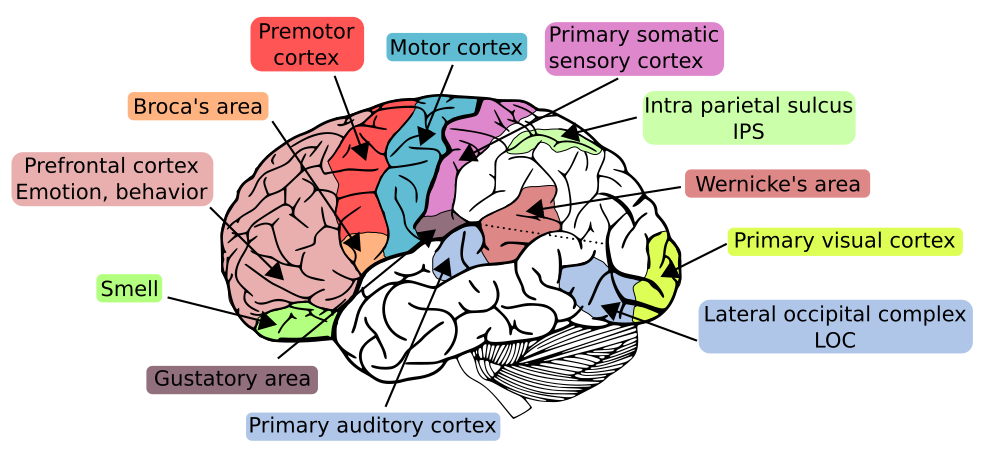
\includegraphics[width=1\linewidth]{figures/brain_function.png}
  \caption{The main functional regions of the human brain (left hemisphere),
and the two regions which are studied in this thesis (LOC and IPS). Adapted
from \url{http://agaudi.files.wordpress.com/}}
\end{figure}
blablablabla
blablablabla
blablablabla
blablablabla
blablablabla
blablablabla
blablablabla
blablablabla
blablablabla
blablablabla
blablablabla
blablablabla
blablablabla
blablablabla
blablablabla
blablablabla
blablablabla
blablablabla
blablablabla
blablablabla
blablablabla
blablablabla
blablablabla
blablablabla
blablablabla
blablablabla
blablablabla
blablablabla
blablablabla
blablablabla
blablablabla
blablablabla
blablablabla
blablablabla
blablablabla
blablablabla
blablablabla
blablablabla
blablablabla
blablablabla
blablablabla
blablablabla
blablablabla
blablablabla
blablablabla
blablablabla
blablablabla
blablablabla
blablablabla
blablablabla
blablablabla
blablablabla
blablablabla
blablablabla
blablablabla
blablablabla
blablablabla
blablablabla
blablablabla
blablablabla
blablablabla
blablablabla
blablablabla
blablablabla
blablablabla
blablablabla
blablablabla
blablablabla
blablablabla
blablablabla
\begin{marginfigure}
    \centering
    \def\svgwidth{\columnwidth}
    \input{figures/neuron.pdf_tex}
    \caption{\textbf{Simplified view of a neuron.} A \textit{neuron} has a cell body
called the \textit{soma}, many regions for receiving information from other neural cells
called \textit{dendrites}, and often an \textit{axon} (nerve
fiber) for transmitting information to other
cells (an axon can be longer than 1 me-
ter in humans) The information in the
axon is transmitted through an electri-
cal signal called action potential, which
is based on the electrical properties of
the neuronal membrane. Adapted from
\url{http://commons.wikimedia.org/}}
\end{marginfigure}

blablablabla
blablablabla
blablablabla
blablablabla
blablablabla
blablablabla
blablablabla
blablablabla
blablablabla
blablablabla
blablablabla
blablablabla
blablablabla
blablablabla
blablablabla
blablablabla
blablablabla
blablablabla
blablablabla
blablablabla
blablablabla
blablablabla
blablablabla
blablablabla
blablablabla
blablablabla
blablablabla
blablablabla
blablablabla
blablablabla
blablablabla
blablablabla
blablablabla
blablablabla
blablablabla
blablablabla
blablablabla
blablablabla
blablablabla
blablablabla
blablablabla

% \section{Resting-state networks}
% \section{Clinical implications}
\begin{figure}[!htbp]
  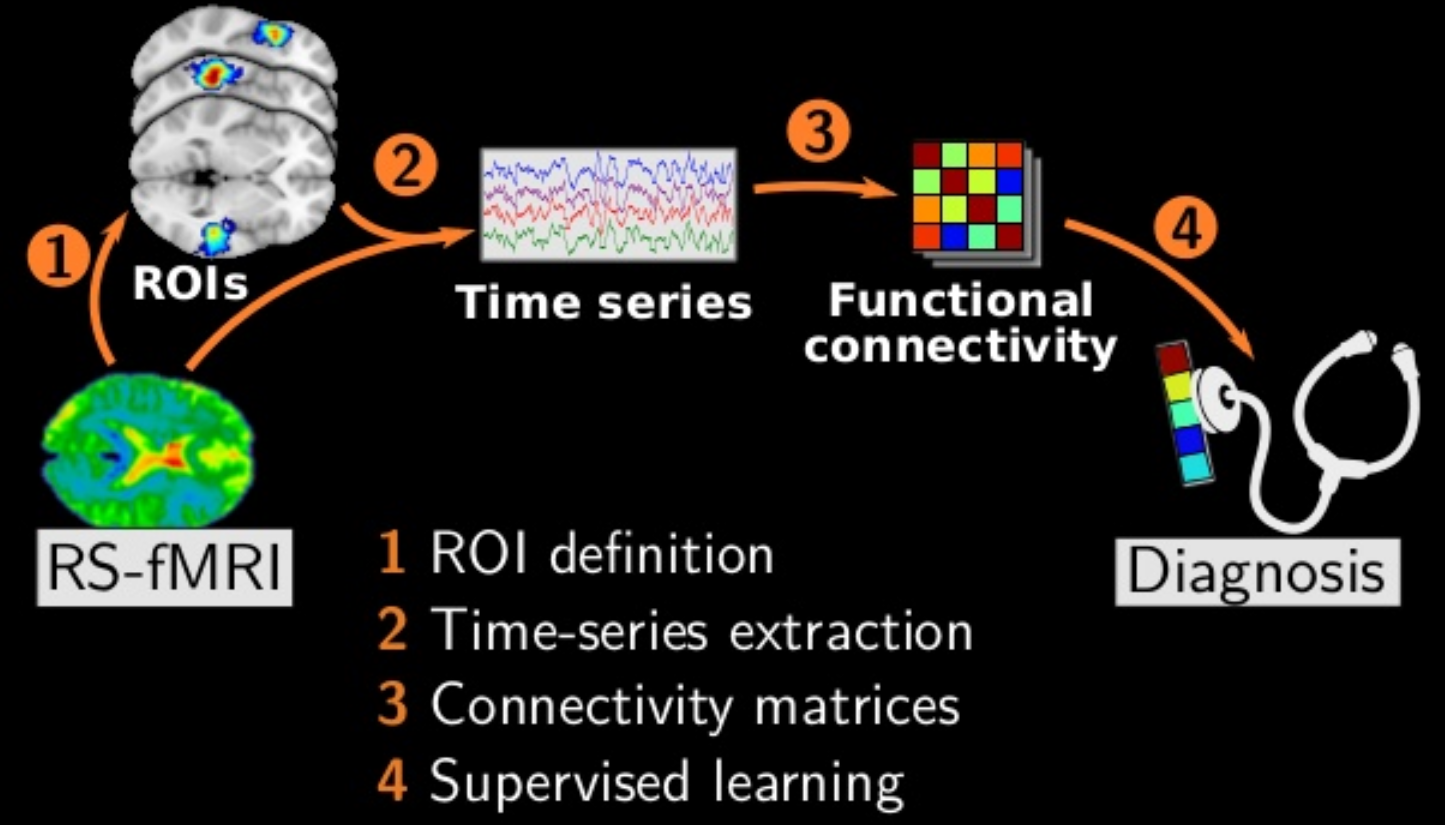
\includegraphics[width=1\linewidth]{figures/big_picture.png}
  \caption{...}
\end{figure}
% \section{The functional brain as a dynamic graph}
\begin{marginfigure}%[!htbp]
  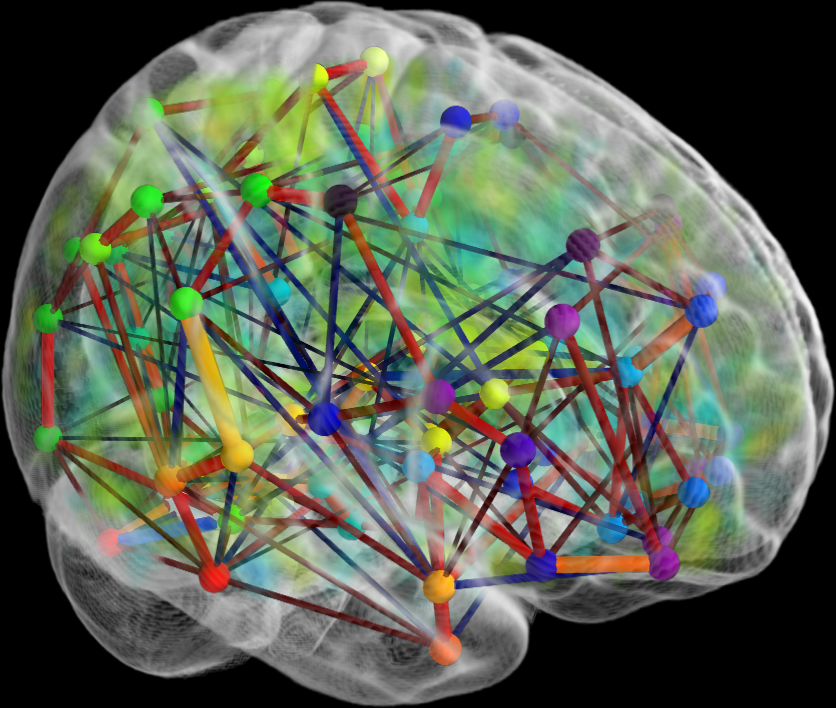
\includegraphics[width=1\linewidth]{figures/connectome.png}
  \caption{...}
\end{marginfigure}

% \section{Task activation as a small perturbation of resting-state networks}

\section{Inter-subject variability in the human brain}
\subsection{Structural variability: the human brain varies in structure, size, and shape}
\subsection{Functional variability: the human brain varies in function}

  
% The first two chapters of this thesis introduce and define concepts that will be developed later on. The other chapters can be read independently of each other. Original contributions and their relative published material are referenced at the beginning of each chapter.



% % This thesis is organized in a way such that Chapter~\ref{chap:intro_fmri} and Chapter~\ref{chap:stats_fmri} are introductory chapters that define the concepts that will be developed in later chapters. The rest of the chapters only depend on these two introductory chapters and can be read independently of each other. 
%  % We propose novel extensions and investigate the theoretical properties of different models. 


% % This thesis is organized in several chapters. Chapter~\ref{chap:intro_fmri} and \ref{chap:stats_fmri} define the concepts that will be developed in later chapters. Chapter~\ref{chap:hrf_estimation} and Chapter~\ref{chap:decoding_ordinal} propose novel applications of machine learning to the analysis of fMRI. Finally, Chapter~\ref{chap:consistency}, which is the most theoretical contribution investigates 


% %Feature extraction and supervised learning on fMRI: From practice to theory

% \vspace{10pt}
% \section*{Chapter \ref{chap:intro_fmri} - Introduction to Functional MRI}

% In this chapter we introduce functional magnetic resonance imaging (fMRI) as a non-invasive functional imaging modality with good spatial resolution and whole brain coverage. We start by presenting briefly the main human brain structures and then reviewing the principal brain imaging techniques in use nowadays, with special emphasis on fMRI.

% The primary form of fMRI measures the oxygen change in blood flow. This is known as the the Blood-oxygen-level dependent (BOLD) contrast. We present a \emph{feature extraction} model known as the \emph{general linear model} (GLM)~\citep{Friston1995} that allows to extract time-independent \gls{activation coefficient}  given the BOLD signal and an experimental paradigm. The difficulty of this process stems from the fact that the BOLD signal does not increase instantaneously after the stimuli onset nor does it return to baseline immediately after the stimulus offset. Instead, the BOLD signal peaks approximately 5 seconds after stimulation, and is followed by an undershoot that lasts as long as 30 seconds. The idealized, noiseless response to an infinitesimally brief stimulus is known as the \emph{Hemodynamic Response Function} (\gls{HRF}).


%  % We describe the main assumptions behind this model: a known form of the hemodynamic response function (HRF) and the linear-time-invariant relationship between the BOLD signal and the neural response. 


% \begin{marginfigure}[-2cm]
% \centering \includegraphics[width=1.\linewidth]{figures/chapter_1/linear_hrf_mini.pdf}
% \caption{The general linear model (GLM) predicts that the expected BOLD response to two overlapping stimuli is the sum of the two independent stimuli. In green, the response to the first stimulus that is located at 1 second. In orange, the response to the second stimulus that appears at 6 seconds. In blue, the predicted BOLD response.}\label{fig:1_lti_hrf} 
% \end{marginfigure}


% % The \emph{Hemodynamic Response Function} (HRF) represents the ideal, noiseless response to an infinitesimally brief stimulus. Different versions of the HRF have been proposed in the literature and in this chapter we examine the characteristic of the HRF used in three different software packages: SPM, AFNI and NiPy.



% In order to estimate the activation coefficients, the GLM assumes a \emph{linear time invariant} (LTI) relationship between the BOLD signal and the neural response. This relationship has been reported in a number of studies and can be summarized as $i)$ \emph{Multiplicative scaling}. If a neural response is scaled by a factor of $\alpha$, then the BOLD response is also scaled by a factor of $\alpha$.
% \mbox{$ii)$ \emph{Additivity}}. If the response of two separate events is known, the signal for those same events is the sum of the independent signals (Fig.~\ref{fig:1_lti_hrf}).
% $iii)$ \emph{Time invariant}. If the stimulus is shifted by $t$ seconds, the BOLD response will also be shifted by this same amount.

% The GLM in its classical formulation assumes a known form for the hemodynamic response function (HRF). In Chapter~\ref{chap:hrf_estimation} we will present an extension of the GLM model that estimates jointly the activation coefficients and the hemodynamic response function.


% % The General Linear Model (\gls{GLM}) makes use of the knowledge of the hemodynamic response function and linear-time-invariant assumption to model the observed BOLD signal. This model states that the BOLD signal can be expressed in terms of a linear combination of the predicted fMRI responses for different stimuli (also denoted \gls{conditions}) plus a noise term (Fig.~\ref{fig:glm1_abs}). 

% % \begin{figure*}[t]
% % \center \includegraphics[width=.8\linewidth]{figures/chapter_1/glm_plain.pdf}
% % \caption{The GLM expresses the observed BOLD signal as a linear combination of regressors plus an error term. Each regressor of the design matrix is the convolution of a reference HRF and the stimulus function, a function that is 1 when the stimulus is present and zero otherwise. Each element of the (unknown) activation coefficeints represent the relative amplitude of a given condition.}\label{fig:glm1_abs}
% % \end{figure*}




% \section*{Chapter 3 - Statistical Inference in fMRI}

% In this chapter we present the statistical methods that will be used for drawing conclusions from fMRI experiments in further chapters. The chapter is divided into two sections. The first section summarizes the basics of statistical hypothesis testing while the second section describes the basics of supervised machine learning.


% Statistical tests can be broadly divided into \emph{parametric} and \emph{nonparametric} tests. Parametric test assume a known probability distribution under the null hypothesis for the distribution parameter that is under consideration. Nonparametric tests do not assume a known form of this probability distribution although they might require some regularity conditions on the distribution such as symmetry. In this chapter  we  describe two parametric statistical tests: the $t$-test and the $F$-test. We will also present a nonparametric test: the Wilcoxon signed-rank test. These tests will be used at different parts of the manuscript. The $t$ and $F$-test will be used to perform voxel-wise inference in section~\ref{subsec:spms} and the Wilcoxon test will be used to compare the performance of different supervised learning models in Chapter~\ref{chap:hrf_estimation}, \ref{chap:decoding_ordinal} and \ref{chap:consistency}.



% \begin{marginfigure}
% \center \includegraphics[width=0.8\linewidth]{chapter_2/spm_visual_auditory_mini.pdf}
% \caption{Statistical Parametric Maps (SPMs) are images with values that are, under the null hypothesis, distributed according to a known probability density function. In the figure, a $t$-map (i.e. the values are distributed according to a Student $t$ distribution) for a contrast of a Visual vs an Auditory task. Thresholded at $p$-value $< 10 ^ {-3}$. It can be seen how the voxels that exhibit a higher significance of this contrast belong to visual areas (red) and auditory areas (blue)}\label{fig:abs_spm}
% \end{marginfigure}

% A notable application of parametric statistical tests to fMRI is the creation of Statistical Parametric Maps (SPMs) (Fig.~\ref{fig:abs_spm}). These are images with values that are, under the null hypothesis, distributed according to a known probability density function, usually Student $t$ or the $F$ distribution. To create such maps, one proceeds by performing a parametric test at each voxel. The resulting statistics are assembled into an image - the SPM. 



% In the second part of this chapter we introduce different supervised learning models that will be used in subsequent chapters. We will consider models that can be estimated as the solution to a minimization problem of the form
% $$
% \argmin_{f \in \mathcal{F}} {\mathcal{R}}_n^{\psi}(f) + \lambda \Omega(f) \quad,
% $$
% where $\mathcal{R}_n^{\psi}(f)$ is a data-fitting term that minimizes a surrogate of the loss function term and $\Omega(f)$ is a regularization term that biases the estimated model towards a set of desired solutions. This way, the model is a trade-off between a data fidelity term and a regularization term. 

% We describe different surrogate loss functions and penalties that have found applications in the context of fMRI analysis. The surrogate loss functions that we describe here are Support Vector Machines, Logistic Regression, Support Vector Regression and Least Squares. The penalties that we consider here are squared $\ell_2$, $\ell_1$, elastic-net ($\ell_2^2 + \ell_1$) and total-variation (TV).



% Finally, we present two applications of supervised learning to reveal cognitive mechanisms in fMRI studies. The first application is commonly known as \emph{decoding} or \emph{mind reading} and consist in predicting the cognitive state of a subject from the activation coefficients. The neuroscientific questions that decoding is able to address are commonly shaped within the statistical hypothesis testing framework. The inference that we want to establish is whether the classifier trained on data from a given brain area of one subject is accurate enough to claim that the area encodes some information about the stimuli. In this setting, the null hypothesis is that a given brain area does not contain stimuli-related information. The ability of the classifier to correctly predict some information about the stimuli is considered a positive evidence in support of the alternate hypothesis of presence of stimuli-related information within the brain activity. As an application of decoding, we present the dataset~\citep{Borghesani2014}, in which we used decoding techniques to establish in which regions of the brain it is possible to decode different aspects of words representing real-world objects.


% A different application is known as \emph{encoding}. Here, the activation coefficients are predicted from some information about the stimuli. The success of an encoding model depends in great measure on our ability to construct an appropriate representation of the stimuli, a transformation that is often nonlinear. For example, \citet{naselaris2009bayesian} constructed two different models for each voxel: a model based on phase-invariant Gabor wavelets, and a semantic model that was based on a scene category label for each natural scene. The authors showed that the Gabor wavelet model provided good predictions of activity in early visual areas, while the semantic model predicted activity at higher stages of visual processing. 


% Encoding and decoding can be seen as complementary operations: while encoding uses stimuli to predict activity,  decoding uses activity to predict information about the stimuli. Furthermore, encoding offers the advantage over decoding models that they can naturally cope with unseen stimuli. For example, \citep{Kay2008} used an encoding model to identify natural images that the subject had not seen before. In this case, the predicted activation coefficients were used to select the image that matched most closely the measured activation coefficients.



% \begin{fullwidth}
% \section*{Chapter~\ref{chap:hrf_estimation} - Data-driven HRF estimation for encoding and decoding models}
% \end{fullwidth}


% % In this chapter we describe a novel method for the simultaneous estimation of HRF and activation coefficients based on low-rank modeling, forcing the estimated HRF to be equal across events or experimental conditions,
% %  yet permitting it to differ across voxels. Estimation of this model leads to
% % an optimization problem that we propose to solve with using a
% % \mbox{quasi-Newton} method, exploiting fast gradient computations. 
% % We compare 10 different HRF modeling methods in terms of encoding and decoding
% % score on two different datasets. These results show that the \mbox{R1-GLM} model
% % outperforms competing methods in both encoding and decoding
% % settings, positioning it as an attractive method both from the points of view
% % of accuracy and computational efficiency.


% As pointed in Chapter~\ref{chap:intro_fmri}, prior to its use statistical inference procedures, the fMRI data usually goes through \emph{feature extraction} process that converts the BOLD time course into time-independent \gls{activation coefficient}. This is commonly achieved using a model known as Linear General Model (GLM). While
% this approach has been successfully used in a wide range of studies, it does
% suffer from limitations. For instance, the GLM commonly
% relies on a \mbox{data-independent} \emph{reference} form of the hemodynamic response function
% (HRF) to estimate the activation coefficient (also known as \emph{canonical} or \emph{reference} HRF). However it is
% known that the shape of this response function
% can vary substantially across subjects, age and brain regions. This suggests that an adaptive modeling of this
%  response function can improve the accuracy of subsequent analysis.



% % At a given voxel, it is expected that for similar stimuli the estimated HRF are also 
% % similar. Hence, a natural idea is to promote a common HRF
% % across the various stimuli (given that they are sufficiently similar), which should result in more robust estimates.
% In this work we propose a model in which a common HRF is shared
% across the different stimuli that we denote \emph{Rank-1 GLM} (R1-GLM). The novelty of our method stems from the observation that the formulation of the GLM  with a
% common HRF across conditions translates to a rank constraint on the vector of estimates. 
% This assumption amounts to enforcing the vector of
% estimates to be of the form $\bfbeta_{\B{B}} = [\mathbf{h} {\beta}_1, \mathbf{h} \beta_2, \cdots, \mathbf{h}
% \beta_k]$ for some HRF $\mathbf{h} \in \RR^d$ and a vector of coefficients $\bfbeta \in \RR^k$. More compactly, this can be written as $\bfbeta_{\B{B}} = \vecop(\B{h}
% \bfbeta^T)$. This can be
% seen as a constraint on the vector of coefficients to be the vectorization of a rank-one
% matrix, hence the name {\it Rank-1 GLM (R1-GLM)}.

% In this model, the coefficients have no longer a closed form expression,
% but can be estimated by minimizing the following loss function. Given $\B{X}_{\B{B}}$ and $\B{y}$ as before, $\B{Z} \in \RR^{n \times q}$ a matrix of nuisance parameters such as drift regressors, the optimization problem reads:
% %
% \begin{eqnarray}\label{eq:abs_r1}
% \begin{aligned}
% \hat{\B{h}}, ~\hat{\bfbeta},~ \hat{\bfomega} ~=~& \argmin_{\B{h}, \bfbeta, {\bfomega}} ~ \frac{1}{2}\|\mathbf{y} - \mathbf{X}_{\B{B}} \vecop(\B{h} \bfbeta^T) - \B{Z} {\bfomega}\| ^2\\
% &\text{subject to } \|\B{B} \B{h}\|_{\infty} = 1 \text{ and } \langle \B{B} \B{h}, \B{h}_{\text{ref}}\rangle > 0 \enspace ,
% \end{aligned}
% \end{eqnarray}

% \begin{figure}[t] \centering
% \includegraphics[width=.9\linewidth]{chapter_3/scores_recovery_1.pdf}
% \includegraphics[width=.9\linewidth]{chapter_3/scores_recovery_2.pdf}
% \includegraphics[width=\linewidth]{chapter_3/scores_decoding_smaller.pdf}
% \caption{\label{fig:abs_identification_scores} Image identification score (higher is better) on two different subjects from the first dataset and average decoding score on the second dataset. In the first dataset the metric counts the number of correctly identified images over the total number of images (chance level is 1/120 $\approx 0.008$). This metric is less sensitive to the shape of the HRF than the voxel-wise encoding score. The benefits range from 0.9\% points to 8.2\% points across R1-constrained methods and subjects. The highest score is achieved by a R1-GLM method with a FIR basis set for subject 1 and by a R1-GLMS with FIR basis for subject 2.

% The metric in the second dataset (decoding task) is Kendall tau. Methods that perform constrained HRF estimation significantly outperform 
% methods that use a fixed (reference) HRF. In particular,
% the best performing method is the R1-GLM with 3HRF basis, followed by the R1-GLMS with 3HRF basis. 
% }
% \end{figure}

% %
% The norm constraint is added to avoid the scale ambiguity between $\B{h}$ and $\bfbeta$
% and the sign is chosen so that the estimated HRF correlates
% positively with a given reference HRF $\B{h}_{\text{ref}}$.
% This ensures the identifiability of the parameters. The optimization problem (Eq.~\eqref{eq:abs_r1}) 
% is {\it smooth} and is convex with respect to $\B{h}$, $\bfbeta$ and $\bfomega$,
%  however it is not {\it jointly convex} in variables $\B{h}$, $\bfbeta$ and $\bfomega$.



% We compare different methods for the joint estimation of HRF and activation coefficients in terms of their score for an encoding and an encoding task. The
% methods we considered are standard GLM (denoted \gls{GLM}), a variant of the GLM that improves estimation in highly correlated settings known as GLM with separate designs (GLMS), Rank-1 GLM (R1-GLM) and Rank-1 GLM with separate designs
% (R1-GLMS). For all these models we consider different basis sets for
% estimating the HRF: a set of three elements formed by the reference HRF and
% its time and dispersion derivative, a FIR basis set (of size 20 in the
% first dataset and of size 10 in the second dataset) formed by the canonical vectors
% and the single basis set formed by the reference HRF (denoted ``fixed HRF''), which
% in this case is the HRF used by the SPM 8 software.

% We consider two different datasets. The first dataset is presented in~\citep{Kay2008} where it is investigated using an encoding paradigm. The second dataset has been presented in~\citep{Jimura_Poldrack_2011} and is naturally investigated using a decoding paradigm. The scores obtained in both datasets can be seen in Figure~\ref{fig:abs_identification_scores}. In both cases, the proposed method (R1-GLM or its variant R1-GLMS) achieve the highest scores. The results presented in this chapter have been published in~\citep{pedregosa:hal-00952554}.





% \vspace{10pt}
% \section*{Chapter~\ref{chap:decoding_ordinal} - Decoding with Ordinal Labels}

% We have presented in Chapter~\ref{chap:stats_fmri} the decoding problem in fMRI. In this setting it is often the case that the target variable consist of discretely ordered values. This occurs for example when target values consists of human generated ratings, such as values on a Likert scale, size of objects (Fig.~\ref{fig:mini_vb}), the symptoms of a physical disease or a rating scale for clinical pain measurement.


% \begin{figure}
% \includegraphics[width=\linewidth]{chapter_4/experiment.png}
% \caption{In \citep{Borghesani2014}, the authors investigated the possibility to predict different aspects of the words subjects were reading while undergoing an fMRI acquisition. One of the problems we investigated is to predict the size of the objects that the words refer to. In this case, the different stimuli are ordered according to their relative size, i.e. hammer is smaller than cow which is smaller than a whale, etc. In this case, the target variable is of \emph{ordinal nature}. }\label{fig:mini_vb}
% \end{figure}


% In this chapter we propose the usage of two loss functions to assess the performance of a decoding model when the target consist of discretely ordered values: the absolute error and pairwise disagreement. These two loss functions emphasize different aspects of the problem: while the absolute error gives a measure of the distance between the predicted label and the true label, the pairwise disagreement gives a measure of correct ordering of the predicted labels. These loss functions lead to two different supervised learning problems. The problem in which we seek to predict a label as close as possible to the correct label is known as \emph{ordinal regression} while the problem of predicting ordering as close as possible to the true ordering of a sequence of labels is traditionally known as \emph{ranking}.  

% The first models specifically tailored for the problem of ordinal regression date back to the proportional odds and proportional hazards models of~\citep{McCullagh1980}. We present three different surrogate loss functions of the absolute error: least absolute error, ordinal logistic regression and cost-sensitive multiclass classification.


% Ranking models were introduced chronologically later than ordinal regression but its popularity has grown in recent years thanks to its applicability to information retrieval (and search engines in particular)~\citep{liu2009learning}. To the best of my knowledge, the first attempt to minimize a convex surrogate of the pairwise disagreement appears is due to~\citet{Herbrich2000}. We consider a model that minimizes a surrogate of the pairwise disagreement: the RankLogistic model. This model can be viewed as a modification of the popular RankSVM model~\citep{Herbrich2000,Joachims2002}.

% The choice of either metric (absolute error or pairwise disagreement) will depend on the problem at hand. For example, in clinical applications it is often desirable to predict a label as close as possible to the true label, in which case the absolute error is the appropriate metric. If however, the purpose of the decoding study is to perform a statistical hypothesis test to claim that the area encodes some information about the stimuli, then the pairwise disagreement can be an appropriate measure~\citep{pedregosa2012learning, Borghesani2014, bekhti:hal-01032909}.




% % We examine the generalization performance of the presented models on both synthetic data and three fMRI decoding problems from two datasets. We conclude that the best performing models is the last absolute error and ordinal logistic when considering the absolute error as metric and the RankLogistic model when considering the pairwise disagreement as metric. 


% \begin{figure*}[t]
% \includegraphics[width=\linewidth]{chapter_4/scores_ordinal.pdf}
% \caption[-4cm]{Generalization errors (lower is better) for three fMRI decoding problems. Two different metrics are used corresponding to the rows in the figure: mean absolute error and mean pairwise disagreement. The $*$ symbol represents the $p$-value associated with a Wilcoxon signed-rank test. This test is used to determine whether a given method outperforms significantly the next best-performing method.}\label{fig:abs_scores_ordinal}
% \end{figure*}

% We examine their generalization error on both synthetic and two real world fMRI datasets and identify the best methods for each evaluation metric (Fig.~\ref{fig:abs_scores_ordinal}). Our results show that when considering the absolute error as evaluation metric, the least absolute error and the logistic ordinal model are the best performing methods. On the other hand, when considering the mean pairwise disagreement the RankLogistic was the best performing method. For neuroimaging studies, this contribution outlines what in our opinion are the best models to choose when faced with a decoding problem in which the target variables are naturally ordered.




% \section*{Chapter~\ref{chap:consistency} - Fisher Consistency of Ordinal Regression \mbox{Methods}}


% Ordinal regression is the supervised learning problem of learning a rule to predict labels from an ordinal scale. Some ordinal regression models have been  used in Chapter~\ref{chap:decoding_ordinal} to model the decoding problem when the target variable consist of ordered values.

% Motivated by its applicability to decoding studies we turn to study some theoretical properties of these methods. The aim is that a theoretical approach can provide a better understanding the methods at hand. For example, \citet{Keerthi2003} proposed two different models for the task of ordinal regression: SVOR with explicit constraints and SVOR with implicit constraints. In that work, the second approach obtained better generalization error in terms of the absolute error loss function. Similar results were obtained by~\citet{lin2006large} replacing the hinge loss by an exponential loss. Yet again, \citet{Rennie} arrived to similar conclusions considering the logistic loss instead. Given these results, it seems natural to ask: is this coincidence or are there theoretical reasons for  this behavior? We will use the result of this chapter to provide an affirmative answer to this last question.
% % By the end of the chapter we will be able to affirmatively answer this question.

% Many of the ordinal regression models that have been proposed in the literature can be viewed as methods that minimize a convex surrogate of the zero-one, absolute (as outlined in Chapter~\ref{chap:decoding_ordinal}), or squared errors. In this chapter we investigate some theoretical properties of ordinal regression methods. The property that we will investigate is known as \emph{Fisher consistency} and relates the minimization of a given loss to the minimization of its surrogate. 

% We consider a rich family of loss functions for ordinal regression. We follow~\citep{Li2007} and determine as admissible loss functions of ordinal regression those that verify the V-shape property, a condition that includes to the best of my knowledge all popular loss functions that have been used in the context of ordinal regression: absolute error, squared error and 0-1 loss. 

% In order to introduce the notion of consistency we must fix some notation. In the supervised learning setting, we are given a set of $n$ observations $\{(X_1,
% Y_1), \ldots, (X_n, Y_n) \}$ drawn i.i.d.~from $X\times Y$ and a \emph{loss
% function} $\ell: \mathcal{Y} \times \mathcal{Y} \rightarrow [0, \infty)$. The goal is to learn from the training examples a measurable mapping called a~\emph{classifier} $h: \XX \rightarrow \mathcal{Y}$ so that the \emph{risk} given below is as small as possible:
% \begin{equation}
% \label{eq:abs_l_risk}
% \mathcal{R}_{\ell}(h) = \EE_{X \times Y}(\ell(Y, h(X)))\quad.
% \end{equation}


% Attempting to directly minimize the risk is not feasible in practice. First, the probability distribution $P$ is unknown and the risk must be minimized approximately based on the observations. Second, due to the non-convexity and discontinuity of $\ell$, the risk is difficult to optimize and can lead to an NP-hard problem. It is therefore common to approximate $\ell$ by a function $\psi: \mathcal{Y} \times \RR^d \to \RR$, called a \emph{surrogate loss function}, which has better computational properties. The goal becomes to find the \emph{decision function} $f$ that minimizes instead the $\psi$-risk, defined as
% \begin{equation}
% \Rpsi(f) = \EE_{X \times Y}(\psi(Y, f(X))) \enspace.
% \end{equation}



% Fisher consistency is a desirable property for surrogate loss functions. It implies that in the population setting, i.e., if the probability distribution $P$ were available, then optimization of the $\psi$-risk would yield a function (not necessarily unique) with smallest possible risk, known as \emph{Bayes predictor} and denoted by $h^*$. This implies that within the population setting, the minimization of the $\psi$-risk and the minimization of the risk both yield solutions with same risk. 
% % In other words, consistency implies that the minimization of the $\psi$-risk, which is usually a convex optimization problem and hence easier to solve converges to a solution with minimal $\ell$-risk.

% \begin{marginfigure}
% \center\textbf{\color{msblue} 0-1 Error}
% \includegraphics[width=1.1\linewidth]{chapter_5/probas_or_01.pdf}
% \vspace{-30pt}\center\textbf{\color{msblue} Absolute Error}
% \includegraphics[width=1.1\linewidth]{chapter_5/probas_or.pdf}
% \vspace{-30pt}\center\textbf{\color{msblue} Squared Error}
% \includegraphics[width=1.1\linewidth]{chapter_5/probas_or2.pdf}
% \caption{
% 	Bayes predictor can be visualized on the probability simplex. Bayes predictor is a function of the conditional probability $\eta_i(x) = P(y\!=i|X\!=\!x)$. The vector $(\eta_1, \ldots, \eta_k)$ belongs to the probability simplex of $R^n$, which is contained within an hyperplane of dimension $k-1$. In the figure, probability simplex in $\RR^3$ is colored according to the output of Bayes predictor.
% }\label{fig:bayes_predictor}
% \end{marginfigure}



% In this chapter we provide a theoretical analysis of the Fisher consistency properties of a rich family of ordinal regression surrogate loss functions, including proportional odds and support vector ordinal regression. The loss functions that we considered can be divided into three categories: regression-based, threshold-based and classification-based. 


% \paragraph{Regression-based loss function. }The \emph{\mbox{regression-based approach}} treats the labels as real values. It uses a standard regression algorithm to learn a real-valued function, and then predicts by rounding to the closest label. In this setting we will examine consistency of two different surrogate loss functions, the absolute error (that we will denote $\psi_{\mathcal{A}}$) and the squared error (denoted $\psi_{\mathcal{S}}$), which are convex surrogates of $\ell_{\mathcal{A}}$ and $\ell_{\mathcal{S}}$, respectively. Given $\alpha \in \RR$, $y \in [k]$, these are defined as
% \begin{equation*}
% \psi_{\mathcal{A}}(y, \alpha) = |y - \alpha|, \quad \psi_{\mathcal{S}}(y, \alpha) = (y - \alpha)^2 \quad.
% \end{equation*}

% We prove that the $\psi_{\mathcal{A}}$ surrogate is consistent with respect to the absolute error and that the $\psi_{\mathcal{S}}$ surrogate is consistent with respect to the squared error. Consistency of $\psi_{\mathcal{A}}$ was already proven by~\citep{Ramaswamy2012} for the case of 3 classes. Here we give an alternate simple proof that extends beyond $k>3$. 

% \paragraph{\bf Threshold-based loss function.} While the regression-based loss functions may lead to optimal predictors when no constraint is placed on the regressor function space as we will see, in practice only simple function spaces are explored such as linear or polynomial functions. In these situations, the regression-based approach might lack flexibility. \emph{\mbox{Threshold-based} loss functions} provide greater flexibility by seeking for both a mapping $f: \XX \to \RR$ and a non-decreasing vector $\btheta \in \RR^{k-1}$, often referred to as~\emph{thresholds}, that map the class labels into ordered real values. In this context of we consider two different families of surrogate loss functions: the \emph{cumulative link} surrogates and the \emph{margin-based} surrogates. The first family of surrogate loss function that we will consider is the \emph{cumulative link} surrogates. In such models the posterior probability is modeled as $P(Y \leq i|X\!=\!x) = \sigma(g_i(x))$, where $\sigma$ is an appropriate link function. We will prove consistency for the case where $\sigma$ is the sigmoid function, i.e., $\sigma(t) = 1/(1 + \exp(-t))$. This model is known as the \emph{proportional odds} model or \emph{cumulative logit} model~\citep{McCullagh1980}. For $x \in \XX, y \in [k]$ and $\alpha_i = g_i(x)$, the proportional odds surrogate (denoted $\psi_{\mathcal{C}}$) is defined as
% \begin{equation}\label{eq:propodds}
% \psi_{\mathcal{C}}(y, \balpha) = 
% \begin{cases}
% -\log(\sigma(\alpha_1)) &\text{ if } y = 1 \\
% -\log(\sigma(\alpha_y) - \sigma(\alpha_{y-1})) &\text{ if } 1 < y < k \\
% -\log(1 - \sigma(\alpha_{k-1})) &\text{ if } y = k.
% \end{cases}
% \end{equation}
% The other family of surrogates, the margin-based surrogates (denoted $\psi^{\ell}_{\mathcal{M}}$) depends on a V-shaped loss function $\ell$ and is given by
% \begin{gather*}
% \label{eq:sum_of_loss}
% \psi^{\ell}_{\mathcal{M}}(y, \balpha) =
% \sum_{i = 1}^{y-1} \Delta \ell(y, i)\phi(\alpha_i) - \sum_{i=y}^{k-1}\Delta \ell(y, i)\phi(-\alpha_i) \enspace.
% \end{gather*}
% where $\Delta\ell(y, i)$ is the forward difference with respect to the second parameter, defined as $\Delta\ell(y, i) = \ell(y,i+1) - \ell(y, i)$. This formulation parametrizes several popular approaches to ordinal regression. For example, let $\phi$ be the hinge loss and $\ell$ the zero-one loss, then $\psi^{T}_{\ell}$ coincides with the Support Vector Ordinal Regression (``explicit constraints'' variant) of~\citep{Shashua, Chu2007}. If instead the mean absolute loss is considered, this approach coincides with the ``implicit constraints'' formulation of the same reference. For other values of $\phi$ and $\ell$ this loss includes the approaches proposed in~\citep{Shashua,Keerthi2003,Rennie,lin2006large}.

% % Since consistency of the threshold-based approach is only proven subject to certain conditions on the underlying probability distribution $P$, we  investigate which are the conditions that guarantee consistency of these surrogates.

% \paragraph{\bf Classification-based loss function} Since we aim at predicting a finite number of labels with a specific loss functions, it is also possible to use generic multiclass formulations such as the one proposed in~\citep{lee2004multicategory} which can take into account generic losses. Given $\phi$ a real-valued function, this formulations considers the following surrogate
% \begin{equation} \label{eq:multiclass}
% \psi_{\mathcal{L}}^{\ell}(y, \balpha) = \sum_{i=1}^k \ell(y, i) \phi(-\alpha_i)
% \end{equation}
% for $\balpha \in \RR^k$ such that $\sum_{i=1}^k \alpha_i = 0$. The prediction function in this case is given by ${\rm pred}(\balpha) = \argmax_{i \in [k]} \alpha_i$. Note however that this method requires the estimation of $k-1$ decision functions. For this reason, in practical settings threshold-based are often preferred as these only require the estimation of one decision function and $k-1$ thresholds.Consistency results of this surrogate was proven by~\citet{Zhang}, so we will limit ourselves to compare their results to our findings of consistency for threshold-based surrogates in Section~\ref{subsec:multiclass}.





% For all the surrogates considered, we either prove consistency or provide sufficient conditions under which these approaches are consistent. Finally, we illustrate our findings by comparing the performance of two methods on 8 different datasets. Although the conditions for consistency that are required by the underlying probability distribution are not necessarily met, we observed that methods that are consistent w.r.t a given loss often outperform other methods that are not consistent with respect to that loss.




% \section*{Chapter \ref{chap:conclusion} - Conclusion and Perspectives}

% We summarize the contributions of this thesis and point out possible extensions that can be considered in the future. These are:

% \begin{enumerate}
% \item For the R1-GLM model introduced in Chapter~\ref{chap:hrf_estimation} we outline a possible direction to improve its computational properties by means of tensor factorizations. 

% \item For the R1-GLM we outline an approach to consider a common HRF at the parcel level. This would allow the model to take advantage of the spatially dependent nature of fMRI. 

% \item The R1-GLM model, being non-convex, comes with no guarantees of convergence to a global optimum for the algorithms considered. We propose to study conditions under which the model is guaranteed to have a unique global optimum.


% \item Some of the results presented in Chapter~\ref{chap:consistency} are valid under restrictive conditions on the probability distribution that generates the data. We propose to extend these results to a more general setting by relaxing some of the conditions imposed to achieve consistency of some models.

% \item We report the possibility to apply ordinal regression methods to 0-1 multiclass classification. Although ordinal regression methods have been initially developed for loss functions that minimize a distance between the labels (typically the absolute error loss), our theoretical results show that some popular models are instead consistent with the 0-1 loss. This suggest that these methods might be competitive within a multiclass classification setting. A potential advantage of these methods compared to other multiclass classification methods is the lower amount of parameters to estimate.
% \end{enumerate}




% % Afin d'estimer les coefficients d'activation, le GLM suppose une relation linéaire invariant de temps (LTI) entre le signal BOLD et la réponse neurale. Cette relation a été rapporté dans un certain nombre d'études et peut être résumée comme i) mise à l'échelle multiplicatif. Si une réponse neurale est réduite par un facteur de α, alors la réponse BOLD est également mis à l'échelle par un facteur de α. ii) d'additivité. Si la réponse à deux événements distincts est connu, le signal de ces événements se ils devaient se produire à proximité dans le temps est la somme des signaux indépendants (Fig. 2.1). iii) Durée invariant. Si le stimulus est décalée de t secondes, la réponse BOLD sera également décalé de ce même montant.
% % Le GLM dans sa formulation classique prend une forme connue pour la fonction de réponse hémodynamique (FRH). Dans le chapitre 5, nous allons présenter une extension du modèle GLM qui estime conjointement les coefficients d'activation et la fonction de réponse hémodynamique.



% \clearpage
\bibliographystyle{plainnat}
\bibliography{bib_all}
